% \Image{Capa do livro (; )}{PNLD2022-008-01.png}

% \Image{Ilustração do livro (EdLab/Renan Costa Lima; EdLab)}{PNLD2022-008-04.png}
% \Image{Ilustração do livro (EdLab/Renan Costa Lima; EdLab)}{PNLD2022-008-05.png}
% \Image{Ilustração do livro (EdLab/Renan Costa Lima; EdLab)}{PNLD2022-008-06.png}


\documentclass[11pt]{extarticle}
\usepackage{manualdoprofessor}
\usepackage{fichatecnica}
\usepackage{lipsum,media9}
\usepackage[justification=raggedright]{caption}
\usepackage[one]{bncc}
\usepackage[edlab]{../edlab}
\usepackage{marginnote}
\usepackage{pdfpages}
\usepackage[printwatermark]{xwatermark}
\newwatermark[pagex=2]{
\includegraphics[scale=3.3]{watermarks/test-a.png}}	% página específica
%\newwatermark[oddpages]{
\includegraphics{watermarks/test-a.png}}			% páginas ímpars
%\newwatermark[evenpages]{
\includegraphics{watermarks/test-a.png}}			% págimas pares
\newwatermark[allpages]{
\includegraphics[scale=3.3]{watermarks/test-b.png}}

\pagecolor{cyan!0!magenta!10!yellow!28!black!28!}

\newcommand{\AutorLivro}{Renan Costa Lima}
\newcommand{\TituloLivro}{As letras e as coisas}
\newcommand{\Tema}{Quotidiano de crianças nas escolas; nas famílias e nas comunidades (urbanas e rurais)}
\newcommand{\Genero}{Prescritivos: instruções; guias; manuais; ciclo de crescimento; ciclo de vida}
%\newcommand{\imagemCapa}{./images/PNLD0001-01.png}
\newcommand{\issnppub}{978-65-89829-05-8}
\newcommand{\issnepub}{978-65-89829-06-5}
% \newcommand{\fichacatalografica}{PNLD0001-00.png}
\newcommand{\colaborador}{Paulo Pompermaier e Renier Silva}

\begin{document}

\title{\TituloLivro}
\author{\AutorLivro}
\def\authornotes{\colaborador}

\date{}
\maketitle

%\begin{abstract}\addcontentsline{toc}{section}{Carta ao professor}
%\pagebreak

\tableofcontents



\section{Sobre o livro}

%27 caracteres
\paragraph{O livro} \textit{As letras e as coisas}, de Renan Costa Lima, traz um abecedário lúdico e divertido para ser explorado com as crianças muito pequenas. O livro foi feito com seu filho, então a grafia das palavras, os desenhos e as formas de colorir seguem a capacidade de representação e coordenação motora características dos bebês e crianças muito pequenas.

%822 caracteres
\paragraph{Descrição} Do A ao Z, a criança acompanha todas as letras do alfabeto nesse livro, com exemplos e ilustrações que reforçam cada letra. Cada dupla de páginas é dedicada a uma letra: do lado esquerdo, fica a letra em formato bem grande e colorida, e do direito um desenho, com a mesma cor, e seu nome escrito, sempre iniciando-se com a mesma letra da página em questão.

Muitos dos desenhos rememtem a elementos da cultura brasileira e do cotidiano das crianças, como abacaxi, cavalo, martelo, queijo, urubu e xícara. Outros, no entanto, referem-se a elementos que as crianças podem ainda desconhecer, sendo, em muitos casos, imaginativos: disco voador, foguete, porcofuso, submarino, vulcão etc. Assim, a criança entra em contato não apenas com o abecedário, mas também com figuras antes desconhecidas e palavras novas, explorando sua capacidade imaginativa e levando a imaginação a outros lugares que não apenas a realidade imediata e cotidiana.



%411 caracteres
\paragraph{Competências} A diversão desse livro é a forma como são grafadas as palavras, como estão traçados os desenhos e coloridas as ilustrações e as letras. Elas seguem os traços típicos de um bebê que está começando a desenvolver a coordenação motora: as letras são coloridas de forma que a cor vaza pela borda da letra, remetendo à dificuldade motora de uma criança, ainda não habituada a empunhar o lápis, a seguir o traçado na hora de colorir. Da mesma forma, as ilustrações apresentam traços simples, e seus nomes são escritos com a caligrafia de alguém que está aprendendo as primeiras letras. Essas características são importantes pois relacionam as primeiras experiências motoras infantis com o hábito da leitura e do livro, pois há uma continuidade entre a capacidade de desenhar/pintar/escrever das crianças e as figuras apresentadas no livro, como se elas próprias pudessem ter feito o livro. Essa associação pode gerar interesse nos pequenos e melhorar o trabalho em cima das competências exploradas pelo livro: iniciar o traçado de marcas gráficas, explorar a coordenação motora, movimentar o corpo para exprimir emoções e desejos, imitar gestos.

%862 caracteres
\paragraph{Aprofundamento} Este material tem a 
intenção de contribuir para que você consiga desenvolver um trabalho aprofundado 
com esta obra na sala de aula. Você encontrará informações sobre a autora, sobre 
o gênero e sobre os temas trabalhados ao longo do livro. Apresentaremos também 
algumas propostas de trabalho para a sala de aula que você poderá explorar livremente, 
da forma que considerar mais apropriada para os seus estudantes. Para a prática 
da Literacia Familiar, oferecemos um guia que pode ajudar nas orientações aos 
responsáveis pela criança, para incentivar o gosto pela leitura e contribuir para 
que os estudantes desenvolvam em casa habilidades que serão importantes no momento 
da alfabetização. Por fim, você encontrará sugestões de livros, artigos e sites 
selecionados para enriquecer a sua experiência de leitura e, 
consequentemente, a de seus estudantes.



\section{Sobre o autor}

\Image{Foto do Autor (Arquivo pessoal)}{PNLD2022-008-02.png}


%532 caracteres
\paragraph{O autor} Renan Costa Lima criou o grupo de pesquisa e produção em artes visuais Transição Listrada, junto com Vitor César e Rodrigo Costa Lima. O grupo desenvolveu suas atividades em Fortaleza de 1999 até 2006. Nesse período fundaram a \textsc{base}, um espaço independente de experimentação em artes visuais, que recebeu artistas locais, nacionais e internacionais como Érika Zíngano, Valéria Américo, Eduardo Verderame, Rodrigo Braga, Graziela Kunsch, Jorge Menna Barreto e Karina Lackner, entre outros. Realizou exposições coletivas e individuais, mostra de vídeos, falas públicas, além de residências artísticas e ponto de encontro entre os artistas locais. O grupo participou de exposições coletivas e individuais, tais como Bienal Ceará de Ponta Cabeça \textsc{ce}, Verbo \textsc{sp}, Mostra \textsc{sesc} de Artes \textsc{sp}, Spa das Artes Visuais \textsc{pe}. Realizou diversas intervenções na cidade de Fortaleza e também esteve em projetos de residência internacional como no Museumsquartier em Viena, que resultou na exposição \textit{Vizinhos}. A \textsc{base} teve como desdobramento o projeto \textit{Base Móvel}, que percorreu cidades no interior do Ceará e São Paulo. 



%313 caracteres
\paragraph{Publicações} Criou o Estúdio Tropical em 2009, um estúdio de design gráfico e vídeo, que desenvolve trabalhos para cinema, música, teatro e dança, fazendo identidade visual, aberturas de filmes, capas de discos, videoclipes e outras atuações no mercado cultural. Nos últimos anos tem atuado na difusão da cultura de cartazes, produzindo peças para bandas, filmes e projetos pessoais. Tal iniciativa resultou na criação, em 2016, da oficina de impressão em risografia Riso Tropical, onde imprime projetos autorais e para terceiros, além de realizar oficinas de impressão.

%358 caracteres
\paragraph{Currículo} Em 2018 inaugurou a \textsc{publica}, espaço independente destinado a cultura e arte no Centro de São Paulo, onde atua ativamente como diretor geral, produtor e nas curadorias de Artes Visuais, Música, Design e Publicações. Com a \textsc{publica} realizou exposições, oficinas, shows, feiras de publicação, residências artísticas, ensaios e demais atividades culturais em diálogo com o entorno do bairro da Vila Buarque, em São Paulo.
 


\section{Sobre o gênero}

%55 caracteres
\paragraph{O gênero} O gênero deste livro é \textit{prescritivo}. 

\Image{No gênero prescritivo, o principal objetivo é instruir o leitor --- assim como a orientação de um dicionário. (Piqsels; Domínio público)}{PNLD2022-008-07.png}

%596 caracteres
\paragraph{Descrição} Como o livro é um abecedário, pode ser classificado no gênero prescritivo, que tem como característica principal instruir o leitor.
Extremamente comum na vida quotidiana, é um gênero presente
sempre que se precisa de uma guia ou uma orientação. São estruturas 
que oferecem padrões: leis, que podem ser jurídicas, como um código
penal, ou gramaticais, como um dicionário ou uma gramática; a constituição
de um país etc. Seu conteúdo é, de alguma forma, imutável, ao menos até que seja
mudado. O significado de uma palavra no dicionário deve continuar o mesmo
até que um novo seja adicionado. Enquanto isso, o texto
estabelecido será aquele que tem valor absoluto.

%603 caracteres
\paragraph{Interação} Talvez o abecedário seja a primeira interação da criança com o gênero prescritivo. De forma lúdica e descontraída, ele faz os primeiros movimentos para instruir a criança no alfabeto, mostrando a ordem das letras, seu uso nas palavras, as iniciais em diferentes palavras etc. Ademais, é um gênero fundamental para a estruturação da sociedade.
Sempre estamos recorrendo a obras prescritivas, em geral de consulta, para
sabermos como devemos agir: seja uma dúvida a respeito da ortografia ou 
dos significados de uma palavra, seja a respeito de um direito ou dever
enquanto cidadão. É de extrema importância, portanto, que as crianças
sejam o mais cedo apresentadas a este gênero, ainda que com a 
devida abordagem lúdica que a idade demanda.

%862 caracteres
\paragraph{Competências} Em um livro como
\emph{As letras e as coisas}, trabalhamos diversas competências relacionadas ao gênero prescritivo. 
Primeiro, há uma apresentação à necessidade de se fazer as coisas de um 
determinado jeito. É o mundo das regras e convenções sociais: há uma ordem correta para as letras no alfabeto, cada palavra se inicia com uma letra diferente e, juntas, elas formam diferentes palavras. As palavras representam coisas, ilustradas ao lado de cada letra, levando-nos a uma segunda competência: a associação entre os traços gráficos, tanto a palavra quanto a letra, e os desenhos. O uso de cores, nesse livro, também facilita o desenvolvimento dessa competência, pois cria outro traço de similitude entre a grafia da palavra e sua representação imagética. Ainda que pareça ser um gênero
limitante, são os conhecimentos fixados nestas obras que permitem a expansão
da criatividade com a garantia de que o outro irá entender já que as convenções são comuns.



\section{Temas}


\subsection{Quotidiano de crianças nas escolas; nas famílias e nas comunidades (urbanas e rurais)}

%136 caracteres
\paragraph{Abordagem} Nesse livro comparecem elementos típicos da vida do estudante, a começar pelas letras. Os exemplos para cada letra também fazem parte de seu universo, facilitando a associação entre letra, palavra e imagem. A forma como as letras são pintadas e como as palavras e desenhos são grafados também aproximam o livro do quotidiano da criança, pois assemelham-se aos traços possibilitados por sua coordenação motora e fina em desenvolvimento.

%206 caracteres
\paragraph{Descrição} O livro pode tanto introduzir os bebês no sistema alfabético, ao apresentar relações primárias entre letras e palavras; quanto possibilitar que exercitem seus traços ao observar o livro e tentar imitá-lo com tinta ou outros materiais.

%275 caracteres
\paragraph{Competências} Este tema relaciona-se, principalmente, ao 
campo da experiência Traços, sons, cores e formas
descrito pela \textsc{bncc}, que explora a capacidade de a criança começar a se expressar com traços gráficos, sons, movimentos corporais e, assim, começar a se exteriorizar de diferentes formas.


\section{Modelagem de aula}
A seguir você encontrará a descrição de uma aula modelo como exemplo 
prático de exploração do livro com estudantes. Esta seção apresentará 
orientações sobre como organizar a sala de aula para receber os 
estudantes, exercitar a interação verbal e prepará-los para o 
momento da leitura.

Em seguida, você encontrará a \textbf{Leitura dialogada}, um 
tópico destinado a te orientar para o momento específico da 
leitura com os estudantes. Por fim, no tópico 
\textbf{Propostas de atividades}, você encontrará ideias 
de práticas que pode explorar com as crianças em sala de 
aula após a leitura. 

Essas atividades podem ser trabalhadas de acordo com a 
disponibilidade do seu cronograma e fique à vontade para adaptá-las 
da forma que achar melhor para os seus estudantes. Cada turma é única 
e o seu conhecimento prático das características de cada aluno será 
essencial para definir a melhor forma de aplicar essas ideias. 

O objetivo deste manual é oferecer algumas ideias 
e inspirações para um trabalho que pode ser desenvolvido tanto 
a curto, quanto a médio e longo prazo. Sinta-se a vontade para 
personalizar a aula e torna-la sua, aplicando seus conhecimentos, sua 
personalidade e aproveite para fortalecer 
seu vínculo com a turma.


\subsection{Antes de ler}

\BNCC{EI01TS02}
\BNCC{EI01TS03}
\BNCC{EI01EO04}
\BNCC{EI01CG01}
\BNCC{EI01CG03}

%Alterar o nível escolar nesse parágrafo.
Como este trabalho será realizado com crianças da \textbf{Creche \textsc{i}}, 
que ainda não têm intimidade com o livro enquanto objeto, você terá o 
papel essencial de mediar este contato. 

Nosso objetivo é que os próprios estudantes possam manusear 
e explorar o livro de forma autônoma, mas, para que isto aconteça, você 
pode ajudar a tornar o caminho mais convidativo com atividades que tenham 
intencionalidade educativa. 

A \textsc{bncc} define intencionalidade educativa como ``organização 
e proposição, pelo educador, de experiências que permitam às crianças 
conhecer a si e ao outro e de conhecer e compreender as relações com a 
natureza, com a cultura e com a produção científica, que se traduzem nas 
práticas de cuidados pessoais (alimentar-se, vestir-se, higienizar-se), 
nas brincadeiras, nas experimentações com materiais 
variados, na aproximação com a literatura e no encontro com as 
pessoas''.\footnote{\textsc{bncc}, página 39}

É importante manter essa intencionalidade em mente não apenas na condução 
das atividades propostas neste manual, mas também para aproveitar as 
oportunidades espontâneas de construir conhecimentos que podem surgir durante 
a interação direta com os estudantes.

\begin{enumerate}
%836 caracteres
\item \textbf{O ambiente}\quad Antes de iniciar o trabalho com o livro, é importante que você 
prepare o ambiente para receber a turma. Como o trabalho com o livro terá 
três momentos (antes, durante e depois da leitura), seria interessante que você 
criasse um ambiente para cada etapa. Nas \textbf{Sugestões de referências complementares} 
você encontrará um artigo que discorre sobre a importância da organização da sala 
de aula para a educação infantil, que pode ser um bom guia para a criação desses 
ambientes.

%413 caracteres
\item \textbf{Contextos}\quad O objetivo desta atividade é trabalhar os sinais gráficos das letras em um contexto dinâmico, envolvendo o sentido da escuta com a música.

\Image{O aquecimento da atividade será feito com música. (Jonas Banhos; CC BY-NC 2.0)}{PNLD2022-008-09.png}

\item \textbf{Materiais}\quad TV ou aparelho de som e imagem; Folha de sulfite A4; Giz de cera e lápis de cor. 

\item \textbf{Desenvolvimento}\quad Coloque o clipe do Grupo Triii - “A E I O U”,\footnote{\url{https://www.youtube.com/watch?v=IFm3SRDPZ60&t=210s}} estimule as crianças a dançarem com o grupo e também a cantar as letras, sendo possível utilizar materiais que fazem som, como chocalhos. Depois do ``aquecimento'' com a música, prepare folhas de sulfite com o desenho bidimensional de algumas letras do alfabeto e peça que as crianças pintem essas letras com giz de cera ou lápis de cor. Em seguida, peça que as crianças compartilhem com a turma as pinturas que fizeram e falem ou balbuciem algum objeto de seu contexto que comece com essa letra. As crianças menores podem ter dificuldades em falar ou pintar as letras, mas é importante que o professor encontre opções viáveis para que essas crianças não deixem de participar, como, por exemplo, pintar junto com a criança segurando em sua mão.

\item \textbf{Perguntas para avaliar}\quad As crianças conseguem repetir o som das letras? Associam a letra com os objetos? A atividade estimulou as crianças a exercitarem a fala?
\end{enumerate}


\subsubsection{A interação verbal} 
Criar situações em que as crianças precisam dialogar diretamente com 
você é uma das práticas mais importantes de Literacia, pois elas estimulam 
o desenvolvimento linguístico, ampliam o vocabulário e reforçam a 
capacidade dos estudantes de compreenderem o que ouvem e se expressarem 
pela fala. O diálogo livre com a criança também reforça sua autoestima, pois 
a faz se sentir ouvida e valorizada pelo adulto, ao vê-lo prestar atenção 
no que ela tem a dizer. Portanto, sempre que possível, reserve um tempo na 
aula apenas para a interação verbal. 

Como esse tipo de interação é espontânea e intimamente atrelada ao 
desenvolvimento de cada estudante, nossas orientações não serão específicas. 
A ideia é que você adapte este momento de acordo com as respostas e os 
repertórios das crianças. É um momento de estreitamento de vínculos e, portanto, 
fique a vontade para ser espontânea e para explorar os tópicos que achar 
mais interessantes para a sua turma.

Inicie as conversas com naturalidade, seguindo os objetos de atenção dos bebês. 
Você pode partir de objetos que estejam olhando ou sons que estão balbuciando 
para iniciar um assunto e incentivar que tentem se expressar. Ainda que nem 
todos os sons coincidam com palavras que conhecemos, continue interagindo, 
pois a intenção aqui é que o bebê perceba que outras pessoas estão respondendo 
à sua tentativa de comunicação. 

Fique atento a todas as formas de expressão: os gestos, as falas, as 
expressões faciais, para onde olham\ldots{} tudo pode ser explorado durante a conversa. 
Demonstre curiosidade sobre eles, seja um ouvinte entusiasmado e incentive que eles 
conversem entre si. Faça perguntas e construa a resposta junto com as crianças, 
a partir dos sons que eles emitem ou de informações que você saiba. 

A seguir, algumas dicas que podem contribuir para que a interação verbal 
seja produtiva em sua sala de aula: 

\begin{enumerate}
\item Sente-se no chão e brinque com eles, estabelecendo 
contato visual. Embora não consigam falar, vocalizações, 
gestos e expressões faciais podem ser boas formas de comunicar.

\item Não se esqueça que a conversa é uma troca e, portanto, 
evite ficar falando sozinho ou desvalorizar as respostas dos 
bebês porque não são palavras completamente articuladas. 
Nunca descarte uma tentativa de comunicação. 

\item Evite utilizar falas negativas que desencorajam o diálogo, 
como ``não pode!'', ``tire a mão'', ``não faça''. Se precisar que a turma 
corrija algum comportamento, explique claramente a razão e 
oriente com calma. Incentive positivamente as crianças e 
destaque o motivo de seus elogios. 

\item Aproveite alguns momentos durante a conversa para chamar 
a atenção das crianças para os sons das palavras e das letras que você 
acabou de usar ou que eles pronunciaram.  

\item Fale sempre com os bebês, pois, apesar de não conseguirem 
falar muito, são capazes de compreender muito.

\item Você pode utilizar a fala materna\footnote{Fala meiga, frequentemente 
utilizada com bebês e crianças pequenas, que alonga as 
vogais das palavras.}, mas não distorça 
a pronúncia correta das palavras e evite diminutivos. Interprete 
os gestos do bebê nomeando seus desejos verbalmente. Se você escutar 
alguma sílaba ou palavra, repita de volta completando e estimule 
positivamente as tentativas de fala. 

\item Explore possibilidades de interação como apontar e 
nomear objetos, pessoas e animais, imitar o bebê ou pedir que 
ele o imite, fazer caretas, jogar beijos, reproduzir sons de 
animais para que repitam, ensinar os nomes de partes do corpo, 
entre outras atitudes que estimulem a comunicação com a criança. 

\item Muitas dessas dicas poderão ser aproveitadas pela 
família durante a prática da Literacia Familiar. Portanto, 
se achar necessário, compartilhe algumas destas orientações 
com as famílias dos estudantes.
\end{enumerate}


\subsection{A leitura dialogada}
Este é o momento em que será realizada a leitura propriamente dita. 
Se possível, crie um \textit{cantinho da leitura} em sua sala de aula. Um 
ambiente confortável, de preferência em que todos se sentem no chão ou 
em pufes para que consigam enxergar as ilustrações do livro que está 
sendo lido e interagir com facilidade. Se houver possibilidade, mantenha 
sempre os livros da turma em uma altura da estante que permita fácil 
acesso para os estudantes ou guarde os livros em uma caixa que as crianças 
possam mexer com autonomia. É importante que elas tenham autonomia para 
acessar os livros e se sintam à vontade para pegá-los sempre que quiserem. 

\Image{É importante que o cantinho da leitura proporcione autonomia para as crianças. (Elza Fiúza/ Agência Brasil; CC BY-NC 2.0)}{PNLD2022-008-08.png}

Outra possibilidade de ambiente para esta leitura, se a escola permitir, 
é efetuar essa leitura ao ar livre, embaixo de uma árvore, onde as crianças 
possam ouvir os sons dos pássaros e sentir o cheiro da grama. Sair da sala 
de aula pode oferecer um ótimo leque de experiências aos seus estudantes e 
reforçar a conexão entre a natureza do livro e a realidade.  

Reserve uma boa parte da aula para o momento da leitura com os estudantes, 
pois é importante que esse momento aconteça sem pressa. O objetivo da 
leitura dialogada é que seja uma leitura em bate-papo. A criança deve 
assumir um papel ativo na leitura, mesmo que ainda não seja capaz de 
ler sozinha. Além de promover o gosto pela leitura, esta prática estimula 
o desenvolvimento da linguagem, enriquece o vocabulário e 
aumenta o conhecimento de mundo.

%Especificar o livro.
No caso de \textit{As letras e as coisas} o diálogo durante a leitura é 
ainda mais importante, pois ajuda os bebês a se familiarizarem com o alfabeto e com as letras com as quais cada palavra apresentada se inicia.
A experiência de leitura, portanto, se apoiará principalmente na sua interação com os bebês. 
Você deve interagir com eles durante toda a 
leitura, fazendo perguntas e partindo de detalhes do livro para 
levantar novas questões. 

O objetivo desta leitura dialogada é estimular a fala e a associação com a grafia e os objetos.
A seguir, algumas orientações para aproveitar este momento: 

\begin{enumerate}
%177 caracteres
\item \textbf{Como começar}\quad Enquanto folheia o livro, o professor deve repetir as letras e as palavras que aparecem no material, pedindo que as crianças façam o mesmo. É importante estimular as crianças a pensarem em outros objetos que começam como a mesma letra que é mostrada no livro, não se limitando à imagem disponível naquele material.
Faça perguntas que estimulem a interação das crianças com o livro:

\begin{itemize}
\item Quem reconhece esse desenho?
\item Que cor é essa?
\item Que letra é essa?
\item Qual palavra começa com a letra A?
\end{itemize}

Estas perguntas te ajudarão a avaliar repertório das crianças. 
Não há problema se as perguntas que você fizer não forem respondidas pelos 
estudantes. Você mesma pode respondê-las de forma simples e articulada. Se achar 
conveniente, peça que repitam algumas palavras com você e valorize tentativas 
de imitar a sua fala. 

\Image{Enquanto o professor lê o livro e compartilha as imagens, pode perguntar aos alunos o que vêem em cada ilustração. (Ministério do Desenvolvimento Social; CC-BY-SA-2.0)}{PNLD2022-008-10.png}

 
%230 caracteres
\item \textbf{Manuseio}\quad Deixe que as crianças manuseiem o livro 
e explore com elas todos os elementos que o compõe.
As crianças mais pequenas podem ter dificuldade em segurar esse material, mas é possível adaptar a atividade trazendo alguns objetos para que elas manipulem (como bola, chocalho, brinquedos) buscando estimular a fala ao repetir o nome de tais objetos. 
Mostre o que é a 
capa e onde estão as páginas. Leia o título do livro em voz alta, seguindo 
a leitura com o dedo, indicando as letras. 

%495 caracteres
\item \textbf{Diálogo}\quad Mantenha sempre o diálogo com as crianças. Para isso, é interessante, a cada dupla de páginas, fazer uma 
pausa para conversar com os estudantes sobre o que estão vendo na ilustração. 
Faça perguntas como: 

\begin{itemize}
\item Que letra é essa?
\item Qual letra vem depois dessa?
\item Que animal é esse?
\end{itemize}

Incentive que apontem nas imagens e nas letras para responder. Se os estudantes não 
conseguirem responder, atraia a atenção deles e aponte 
para a resposta. Incentive que apontem em seguida. 

%346 caracteres
\item \textbf{Escuta}\quad Elogie atitudes positivas, como 
tentar tomar o papel central na leitura. Se os estudantes tentarem 
tomar o seu lugar e começar a falar sobre as letras e palavras do livro --- com palavras já articuladas 
ou não --- valorize e escute com atenção o que estiverem falando. Mas não 
force a leitura. Se as crianças estiverem cansadas, faça outra atividade 
e retorne depois. 

%935 caracteres
\item \textbf{Leitura}\quad Faça perguntas e comentários que aumentem o 
interesse e aticem a curiosidade das crianças sobre o livro. Faça 
perguntas ou comentários como: 

\begin{itemize}
\item Quem se lembra de outra palavra com a letra A?
\item Quem já viu um animal igual a esse?
\item Que cor engraçada essa do porco!
\end{itemize}

Não tenha pressa em passar as páginas. Deixe que os estudantes 
observem as ilustrações e dê tempo para que construam suas imagens 
mentais da história que está sendo narrada. 

Dê emoção 
à leitura. Invente diálogos entre as figuras ilustradas --- ou mesmo entre as letras ---, crie uma voz para 
cada uma, capriche nas expressões faciais enfatize cada sílaba da palavra lida.
Deixe-se guiar pela atenção das crianças, mas se perceber que 
elas estão dispersas ou saltando aleatoriamente as páginas, ajude-as 
a retornar à narrativa. Crie um ambiente amigável onde a criança 
se sinta à vontade para fazer perguntas e comentários durante a leitura.

%382 caracteres
\item \textbf{Interação}\quad Leia o nome das ilustrações do livro, passando o dedo pela palavra enquanto lê e, depois, apontando para o desenho que representa a palavra.
Destaque os sons de algumas 
palavras. Interrompa a leitura em alguns momentos e peça que 
os estudantes repitam palavras. Se possível, 
leia as mesmas palavras várias vezes ou explore as imagens em uma ordem 
diferente, construindo uma nova narrativa com os estudantes. 

\item \textbf{Perguntas para avaliar}\quad A criança demonstra interesse pelo material? As crianças menores conseguem explorar os materiais e balbuciar palavras e sons? As crianças maiores conseguem pensar em palavras que começam com a letra em questão?
\end{enumerate}


\subsection{Propostas de atividades}

\BNCC{EI01TS03}
\BNCC{EI01EO03}
\BNCC{EI01EO06}
\BNCC{EI01CG01}
\BNCC{EI01CG03}
\BNCC{EI01EF02}

\begin{enumerate}
%700 caracteres
\item \textbf{Como começar}\quad Após a leitura dialogada, é hora de criar 
atividades que proporcionem aos estudantes experiências novas a partir do livro 
que acabaram de conhecer. Nesta idade é fundamental explorar os sentidos do bebê e 
ajudá-lo a experimentar o que acabou de conhecer de formas diversas. Se achar 
conveniente, convide os estudantes a se sentarem nas carteiras para este terceiro 
momento, pois muitas atividades que serão realizadas exigem apoio para escrever 
ou manipular objetos. É interessante, por exemplo, explorar as letras do alfabeto em associação com o nome dos animais e os sons que eles emitem.
Assim, a criança percebe a conexão entre as imagens que acabou de ver e os elementos da realidade. Para ajudar a traçar 
essa relação, separe previamente desenhos de animais relacionados ao livro e, se possível, algum aparelho de som para reproduzir uma música relacionada à tarefa e o som dos animais. 

%650 caracteres
\item \textbf{O ambiente}\quad A atividade pode ser realizada em dois ambientes distintos. Primeiro, na sala de aula, onde o professor pode dispor ilustrações e desenhos de animais ao lado de uma letra bem grande que represente a primeira letra do nome do animal. É interessante deixar esses desenhos ao alcance das crianças para que possam manuseá-los.
O segundo momento da atividade pode ser realizado em um espaço aberto, pois envolve música e, assim, é interessante dançar e brincar com as crianças, estimulando a consciência corporal e relacionando-a ao universo das letras e do alfabeto.

%950 caracteres
\item \textbf{A atividade}\quad Leve material impresso em folha que contenha figuras de animais e a primeira letra que corresponde ao seu nome. Por exemplo: a imagem de um gato com a letra G ao lado. Deixe esse material exposto para que as crianças possam ver. Ao chamar atenção para a imagem de um animal, coloque em aparelho o som que esse animal faz e peça que as crianças imitem este som, por exemplo: gato = miau. Escolha ao menos 5 animais para esta atividade. Em seguida, leve as crianças para um espaço externo e coloque a música do grupo Tiquequê, ``Se eu fosse\ldots''.\footnote{\url{https://www.youtube.com/watch?v=YNwT0vilGIs}.} É importante que o professor aprenda a coreografia e estimule as crianças a dançar ao som da música, imitando os gestos dos animais, como no vídeo. 

%550 caracteres
\item \textbf{Interação}\quad O livro pode e deve ser 
manipulado pelos estudantes. Incentive que eles façam perguntas, atice sua curiosidade em relação aos animais apresentados e seus sons e proponha que imaginem juntos como é o som 
de outros animais. Quando as crianças propuserem um som, imite o barulho que 
fizeram e interpretem uma conversa entre os animais fazendo apenas 
sons. Se os bebês ainda não conseguirem inventar sons para os animais, faça 
o som primeiro e peça que imitem, valorizando as tentativas.

\item \textbf{Perguntas para avaliar}\quad As crianças conseguem utilizar o movimento corporal para imitar os movimentos propostos? Percebem a diferença entre o som de um animal e de outro? 
\end{enumerate}


\section{Literacia familiar}
O \textsc{pna} dá destaque especial para a importância do envolvimento da família 
no processo pedagógico nesta faixa etária e denomina Literacia Familiar o conjunto 
de experiências e práticas relacionadas à linguagem (oral, escrita ou lida) vivenciadas 
com os cuidadores. 

Essas estratégias podem começar a ser colocadas em prática desde a 
gestação e continuar até o final da adolescência. São práticas simples e divertidas 
que estimulam o desenvolvimento de quatro atividades fundamentais: ouvir, falar, 
ler e escrever que criam momentos de afeto e interação para a família. 

Para que esse trabalho conjunto entre escola e família funcione, é 
fundamental que a escola esteja em constante diálogo com os responsáveis e 
você consiga orientá-los. Um grupo em aplicativos de mensagens instantâneas ou um 
grupo de e-mails são saídas viáveis para que a comunicação se estabeleça e pode ser 
uma forma útil das famílias compartilharem suas vivências e trocarem sugestões 
de abordagens, sempre contando com a sua mediação. 

Com o objetivo de incentivar 
a prática da \textit{literacia familiar}, se possível, organize um rodízio entre os familiares 
das crianças para emprestar o livro da biblioteca da turma. Neste caso, crie um caderno 
de registro e estabeleça períodos para cada família ficar com o livro. É importante 
que os familiares compreendam a seriedade deste compromisso, pois o livro pertence 
ao acervo da sala e, portanto, deve ser bem cuidado e devolvido na data acordada. 

Se não for possível garantir o acesso direto dos cuidadores da criança ao livro, 
grave um vídeo direcionado a eles, contando a história e apresentando algumas 
das ilustrações. O importante é que os familiares saibam com clareza qual livro 
está sendo trabalhado, a história contada e se sinta seguro para explorar as temáticas 
do livro com a criança. Orientações claras e a manutenção do canal de comunicação com 
os responsáveis é essencial para que eles se sintam seguros e à vontade para fazer perguntas 
se tiverem dúvidas. 

Neste manual, você encontrará algumas práticas que podem ser 
recomendadas aos familiares para ajudá-los a expandir e aprofundar o trabalho 
que você iniciou em sala de aula.


\subsection{Importância da leitura}
Na escola, aprendemos a ler letras, mas é importante ter em mente que nós 
lemos o mundo desde muito pequenos: “lemos” os animais que passam pelos nossos 
quintais, a expressão no rosto dos nossos familiares, as cores que pintam o céu 
em um fim de tarde. 

Vamos aprendendo, ao longo da vida, a interpretar acontecimentos 
e sons que escutamos e a utilizá-los para nossa comunicação. Aprender a ler textos e 
escrevê-los expande a nossa leitura do mundo, pois permite que sejamos capazes de 
interpretar um código e experimentar, a partir dele, novas experiências e conhecimentos. 

O simples contato com os livros já permite um leque grande de sensações: 
sentimos as texturas, as formas, vemos as cores do livro, escutamos o som da página 
virando e o som da voz do narrador, se a história estiver sendo lida em voz alta. Para um 
bebê, são experiências que podem contribuir diretamente com o desenvolvimento psicomotor 
e cognitivo. 

Nosso papel, enquanto mediadores de leitura, é contribuir para que essas 
sensações sejam associadas a momentos positivos, de construção de 
conhecimento e exercício de imaginação. 

Com os livros, podemos conhecer mais da história humana, descobrir informações 
novas sobre sociedades diferentes da nossa, imaginar situações e contextos inéditos 
para nós e aumentar o nosso repertório. São por meio deles que melhoramos nossa 
capacidade de interpretação, de expressão, de análise e senso crítico. Boas habilidades 
leitoras podem contribuir para o desenvolvimento de um estudante em todas as outras 
disciplinas, pois exercem influência direta na forma como absorvemos e 
construímos conhecimento.


\subsection{O papel da família na formação do leitor}
A família é peça fundamental na formação do leitor, pois é ela quem primeiro 
ensina a criança a ler. Não apenas os textos escritos, mas a ler o mundo, a 
interpretar os estímulos que a cercam, a construir seu próprio vocabulário e a 
comunicar seus pensamentos e necessidades. Na fase em que estão, os bebês 
absorvem o conhecimento com voracidade e tentam aprender a se comunicar. 

O universo das letras é muito presente na vida das crianças antes mesmo de sua 
entrada na escola. Aparece nas histórias e ilustrações do livro que o cuidador 
lê ao colocá-la para dormir, nas situações em que vê os responsáveis se comunicarem 
pela escrita ou nos textos que podem permear seu cotidiano (nos outdoors, na 
televisão, no celular, manuais de instrução entre outros). 

Os familiares têm, 
portanto, uma ótima oportunidade de apresentar a leitura com leveza, de forma 
prazerosa, associado ao contexto em que a criança vive e à momentos de diversão. 
Você poderá orientar os pais nesta tarefa, ensinando-os com este guia a aproveitar 
as oportunidades para trabalhar a Literacia com a criança.


\subsubsection{Práticas de literacia familiar} 

São muitas as experiências que a prática da \textit{literacia familiar} 
pode oferecer às crianças. A seguir, explicamos cada uma delas para que você possa, 
se achar necessário, compartilhar com os responsáveis enquanto estiver orientando-os: 

\paragraph{Interação verbal} Aumentar a quantidade de conversas com as 
crianças, fazendo perguntas para incentivar o diálogo.

\paragraph{Leitura dialogada} Interagir com a criança durante a leitura 
em voz alta, criar expectativa sobre o livro, chamar a atenção para detalhes 
das ilustrações e comentar o enredo.

\paragraph{Narração de histórias} Interagir com a criança enquanto 
estiver narrando uma história, por exemplo, incluindo-a na ação, utilizando 
marionetes ou permitindo que ela complete a narrativa.

\paragraph{Contatos com a escrita} Apresentar as letras para as 
crianças, incentivar que tentem escrever ou ler, ajudá-los a desenhar letras, 
entre outras formas de incentivar o contato com as palavras.

\paragraph{Atividades diversas} Qualquer atividade com a criança 
pode ser utilizada para contribuir para a alfabetização. Jogos, brincadeiras, 
instrumentos musicais, canto, dança, passeios e viagens oferecem boas 
oportunidades de aprendizado.

\paragraph{Motivação} Atitudes que motivem as crianças à envolver-se com 
o mundo da leitura e da escrita.

\subsection{Exercitando a literacia familiar}

\BNCC{EI01ET03} 
\BNCC{EI01EF03} 
\BNCC{EI01EF05} 
\BNCC{EI01EF07} 
\BNCC{EI01EF08} 

\begin{enumerate}
%700 caracteres
\item \textbf{Como começar}\quad Uma primeira forma de aproximar a família do trabalho com o livro e a criança é explorar o proposto na atividade de pré-leitura. Conversar com os pais sobre a importância de desenvolver a expressão corporal e como fazo-la ao mesmo tempo em que se explora o alfabeto e as figuras do livro. Pode-se começar pedindo aos familiares que coloquem a música\footnote{\url{https://www.youtube.com/watch?v=IFm3SRDPZ60&t=210s}.} para ouvir em casa e dancem e cantem com as crianças.
Se achar conveniente, compartilhe com 
os familiares algumas dicas das seções Interação verbal 
e Leitura dialogada e as indicações nas Referências Complementares 
para ajudá-los a explorar as possibilidades oferecidas pelo livro. 

%650 caracteres
\item \textbf{Leitura}\quad A família pode continuar 
explorando os temas apresentados pelo livro. Os familiares podem explorar 
elementos do cotidiano que se relacionam à história e indicar a conexão 
entre o que viram na ilustração e a realidade.
É importante conversar com a família para explicar a importância do estímulo verbal com a criança, mesmo a mais pequena. Neste caso, é possível sugerir conversas no momento da alimentação, do banho, ou de outra atividade cotidiana, buscando repetir o nome dos objetos e ações que o bebê tem contato. 
Oriente-os a mostrar as 
árvores, animais e outros elementos do cotidiano para os bebês, utilizando-os para reforçar as letras, repetindo pausadamente o nome das palavras.

%1073 caracteres
\item \textbf{Instrução}\quad Informe aos pais o propósito do livro, ressaltando como os desenhos, palavras e coloridos da obra aproximam-se do universo infantil e de suas capacidades motoras finas. Solicite aos pais que tentem brincar, quando possível, com o livro e a criança. Eles podem pedir, por exemplo, que a criança tente manusear tintas ou outros objetos que gravam para tentar imitar as figuras e os traços do livro.
Desdobre com os pais, igualmente, alguns pontos tratados na sugestão de atividade.
Explique a importância de associar as letras aos animais e seus sons e peça que a família estimule as crianças a perceber e repetir esses sons.
Os pais podem trazer outras narrativas, imagens e palavras para apresentar à criança que, mesmo pequena, consegue perceber a diferença entre 
as formas de abordar o livro em sala de aula e na sua casa, e elementos de uma linguagem podem ajudá-la a compreender sentidos e perceber detalhes de outra. Se possível, depois da leitura, oriente que voltem ao livro e retomem as palavras e figuras apresentadas ali, reforçando e estimulando novamente a associação entre a letra e a figura.

Outra opção é entregar o livro para a criança e pedir que ela conte 
sobre o que aprendeu na aula para que o familiar ouça. Mesmo que a narrativa não pareça 
completa para o adulto, é importante que ele ouça com atenção e 
valorize todas as tentativas da criança. Afinal, ao tentar recontar, 
ela manipulará o livro, treinará a coordenação motora, conhecerá as texturas 
do objeto e poderá imitar a forma como o adulto 
lê as palavras, treinando a fala. 
\end{enumerate}

 
\section{Sugestões de referências complementares}

\subsection{Livros} 

\begin{itemize}
\item LINS, Guto. Livro infantil? projeto gráfico, metodologia, subjetividade. São Paulo: Rosari, 2002.
Livro que aborda a importância das escolhas visuais (ilustração, projeto gráfico, lettering) na literatura infantil.  

\item HUNT, Peter. Crítica, teoria e literatura infantil. São Paulo: Cosac Naify, 2010.
Livro sobre crítica de literatura infantil que contêm definições de livro ilustrado e livro imagem. 
\end{itemize}

\subsection{Artigos}

\begin{itemize}
\item SARDELICH, Maria Emilia. Leitura de Imagens, Cultura Visual e Prática Educativa. 
In: Cadernos de Pesquisa. V.36, n.128, p.451-472, mai/ago.2006. Disponível em: \url{https://www.scielo.br/pdf/cp/v36n128/v36n128a09}. 
Acesso em 29 abr 2021. 
Artigo acadêmico que discorre sobre a importância de trabalhar cultura 
visual na educação na sociedade contemporânea. 

\item PRANKE, Marha Elfrida. Organização dos espaços da sala de aula na Educação Infantil. Disponível em: \url{http://centraldeinteligenciaacademica.blogspot.com/2016/04/organizacao-dos-espacos-da-sala-de-aula.html}. Acesso em 04 mai 2021. 
Artigo acadêmico que discorre sobre a importância da rotina e de criar ambientes dentro da sala de aula na Educação Infantil.  
\end{itemize}

\subsection{\textit{Sites}}

\begin{itemize}
\item Vídeos “Conta pra mim” no site do PNA. Disponível em: \url{http://alfabetizacao.mec.gov.br/contapramim}. 
Acesso em 13 abr. de 2021.
Página do MEC com vídeos sobre leitura dialogada que visam incentivar a Literacia Familiar. Muitas das 
técnicas, explicações e materiais disponíveis nessa página podem ser utilizados em aula, mas o site também 
pode ser uma ótima indicação para ajudar a direcionar os cuidadores dos estudantes a praticar 
a literacia familiar e leitura dialogada.

\item Vídeo “Livros de imagem: como utilizar com as crianças?” do canal Conta Outra. Disponível em Youtube. 
Acesso em 14 abr. 2021. 
Neste vídeo, a pedagoga Bel explica o que são livros de imagem e faz sugestões para mediar a leitura com 
crianças. Se você achar conveniente, esse vídeo pode ser recomendado aos familiares da criança 
para inspirá-los na leitura dialogada. 

\item Site da ilustradora Taisa Borges. Disponível em https://taisaborges.com/. Acesso em 13 abr. 2021. 
Site da autora do livro que contém algumas informações sobre ela e amostras de todos os livros que ela publicou. 
Você pode selecionar algumas ilustrações no site para explorar com seus estudantes em sala de aula. 

\item 7 receitas de tinta comestível para bebês. 
Disponível em \url{https://www.tempojunto.com/2015/09/26/7-receitas-de-tinta-comestivel-para-bebes/}. 
Acesso em 29 abr. 2021. 
Neste site você encontrará diversas receitas de tintas comestível que você pode produzir 
para utilizar com os estudantes em atividades na sala de aula. 
\end{itemize}

\subsection{Para os estudantes}
\begin{itemize}
\item Música “A coruja” do canal Heróis do coração. Disponível em Youtube. Acesso em 28 abr. 2021. 
Canção de ninar sobre uma coruja que pode ser trabalhada tanto em sala de aula quanto pelos familiares em casa. 
A melodia familiar e a letra simples permitem a exploração de sons e ritmos pelos bebês. 

\item Música “A Corujinha” de Elis Regina. Disponível em Youtube. Acesso em 28 abr. 2021. 
A letra desta canção se aproxima bastante da história da fábula que inspirou o livro de Taisa Borges, 
pois fala sobre uma corujinha feia. No link há uma animação que pode ser explorada junto com as crianças. 

\item Livro de imagens Telefone sem fio, de Ilan Brenman e Renato Moriconi. Companhia das Letrinhas, 2010. 
Se houver interesse em trabalhar mais uma narrativa visual com as crianças, este livro pode ser uma boa opção. 
As ilustrações grandes e ricas em detalhes atrairão a atenção dos bebês e incentivarão que brinquem entre si. 
\end{itemize}


\section{Bibliografia comentada}

\subsection{Livros}

\begin{itemize}
\item BRASIL. Ministério da Educação. Base Nacional Comum Curricular. Brasília, 2018.
Consultar a BNCC é essencial para criar atividades para a turma. Além de especificar 
quais habilidades precisam ser desenvolvidas em cada ano, é fonte de informações sobre 
o processo de aprendizagem infantil. 

\item BRASIL. Ministério da Educação. Secretaria de Alfabetização. Conta pra mim: Guia de Literacia Familiar. 
Brasília: MEC, SEALF, 2019. Disponível em: \url{http://alfabetizacao.mec.gov.br/images/conta-pra-mim/conta-pra-mim-literacia.pdf}
Este guia é voltado aos pais e oferece explicações em uma linguagem bastante acessível e detalhada as práticas de Literacia Familiar, 
como praticar leitura dialogada, como narrar histórias, como exercitar interação oral, formas de proporcionar contatos com a escrita à criança etc. 
 
\item BRASIL. Ministério da Educação. Secretaria de Alfabetização. PNA Política Nacional de Alfabetização/Secretaria 
de Alfabetização. Brasília: MEC, SEALF, 2019.
Um guia fundamental para trabalhar pré-alfabetização e alfabetização de estudantes, que ressalta a importância da Literacia e da Numeracia. 

\item VAN DER LINDEN, Sophie. Para ler o livro ilustrado. São Paulo: Cosac Naify, 2011.
Livro sobre as particularidades do livro ilustrado, que apresenta as diferenças entre o livro ilustrado e o livro com ilustração. 
\end{itemize}

\subsection{Artigos}

\begin{itemize}
\item COSTA, A. C. C.; SANTOS NETO, J. A.; BORTOLIN, S; PEREIRA, Ana Paula. O livro de imagem e a mediação na escola. 
In VII SECIN, Universidade de Londrina. Disponível em \url{http://www.uel.br/eventos/cinf/index.php/secin2017/secin2107/paper/viewFile/445/296}. 
Acesso em 29 abr 2021. 
Esse artigo reflete sobre a importância de se apresentar livros de imagem para os estudantes na escola para que as crianças aprendam a ler imagens. 

\item NANNINI, P. B. R.; MEDEIROS, J. P. S.; RIBEIRO, J. M. Leitura em cena: Vivências em sala de aula com livro de imagens. 
Literartes, n. 3, p. 82-101, 2014. DOI: 10.11606/issn.2316-9826.literartes.2014.89204. 
Disponível em \url{https://www.revistas.usp.br/literartes/article/view/89204/92115}. Acesso em 29 abr. 2021. 
Artigo acadêmico sobre um trabalho utilizando o mesmo livro de imagem com crianças da educação infantil e ensino médio. 
É uma forma interessante de perceber que a leitura de imagens pode ser explorada com qualquer faixa etária. 
\end{itemize}

% 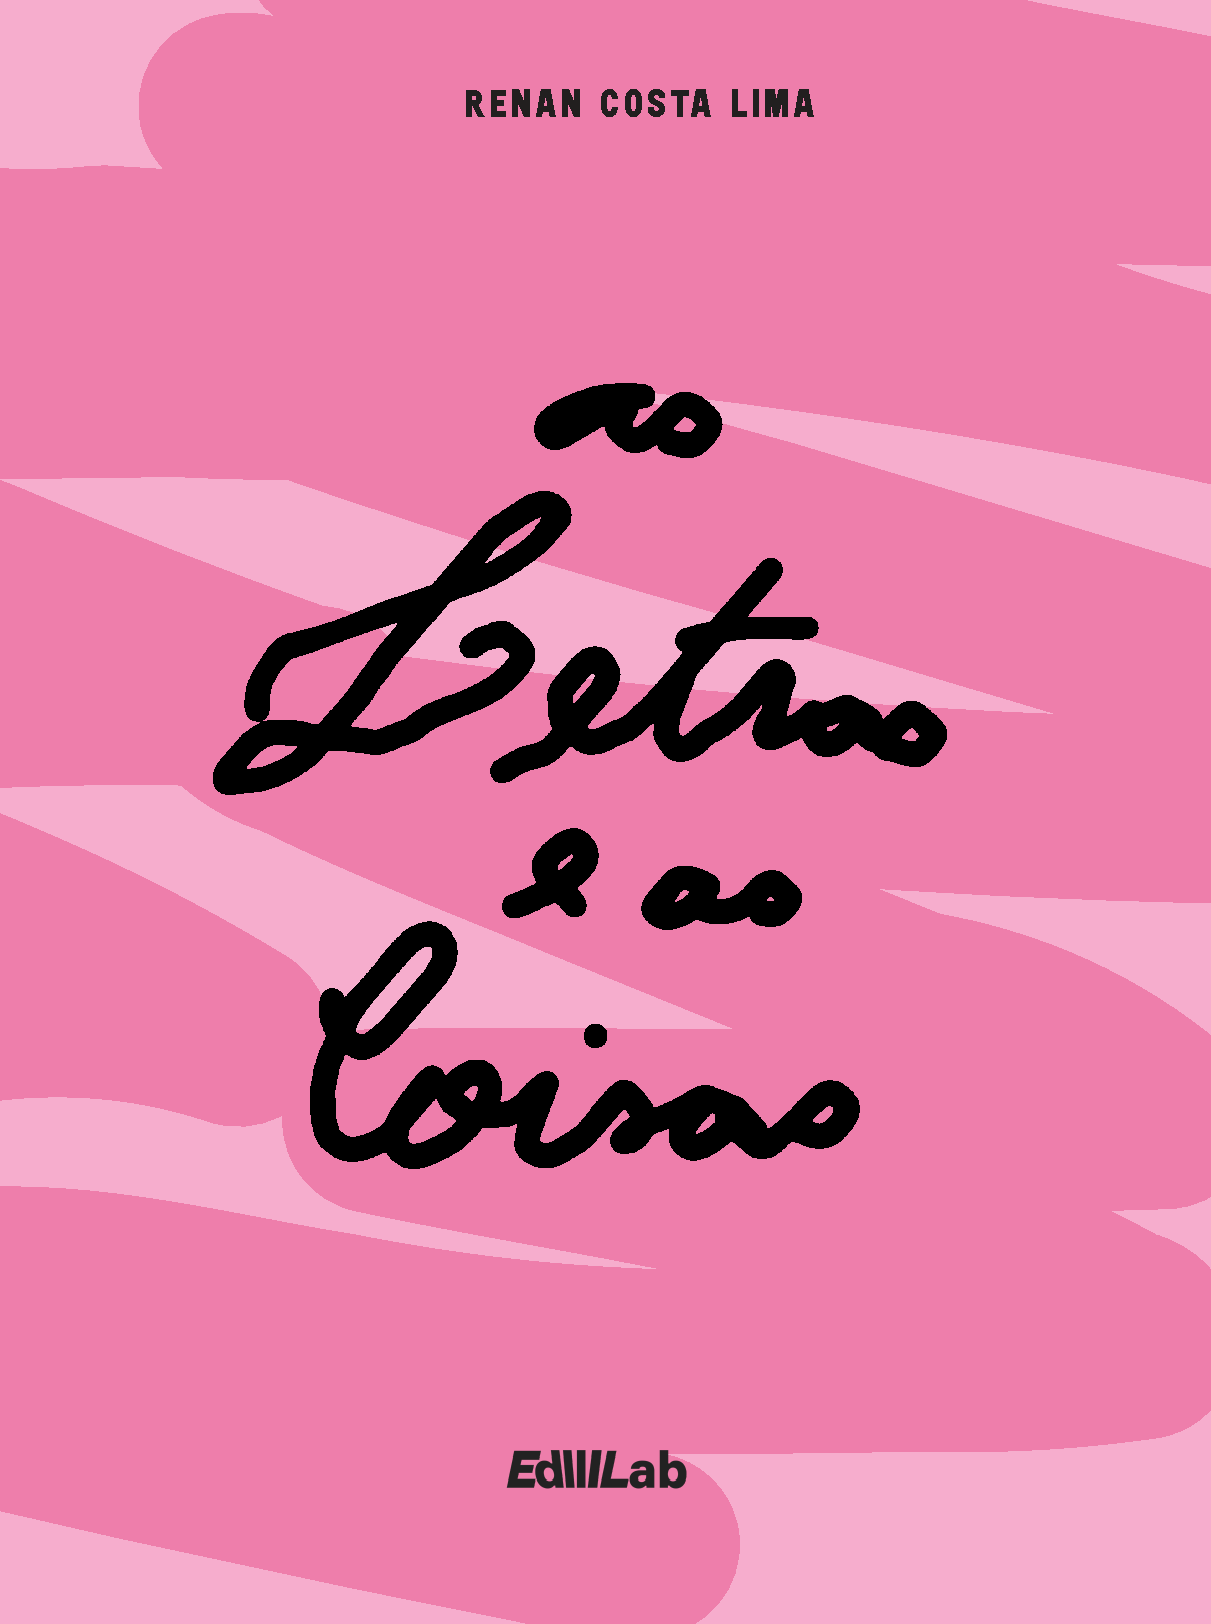
\includepdf[nup=2x2, 					% grid
			% offset=-15mm -5mm, 		% posição
			% scale=.8, 				% tamanho da página
            % delta=4mm 4mm, 			
            % frame,
            % pages={1-4}]{pdfs/PNLD2022-008_MIOLO.pdf}

\end{document}
